\FloatBarrier
\section{Specifica dei meccanismi di comunicazione}
\label{sct:specifica_meccanismi}

I meccanismi di message passing presi in considerazione sono canali unidirezio\-nali di forma simmetrica e asimmetrica in ingresso, entrambi con grado di asincronia unitario e tipo di dati trasmessi ``riferimento alla memoria condivisa''. \\
Viene fornita una descrizione astratta di questi meccanismi e delle relative primitive. Nelle sezioni successive sono descritte le implementazioni che fanno uso di due diversi supporti architetturali: la memoria condivisa con l'uso della gerarchia cache, e la rete di interconnessione tra i PEs. 

\subsection{Descrizione dei canali al livello firmware}
\label{sct:ch_firmware}
Prima di descrivere l'implementazione delle forme di comunicazione considerate, viene descritto brevemente il protocollo tipico per realizzare la comunicazione di unit\`a di elaborazione firmware in modo indipendente dal tempo \cite{vanneschi2009architettura}. Le idee alla base di questo protocollo sono utilizzate per realizzare dei meccanismi efficienti e ottimizzati sull'architettura di \tile.
\begin{figure}[!b]
  \begin{subfigure}[b]{.5\textwidth}
    \centering
    \resizebox{.8\columnwidth}{!}{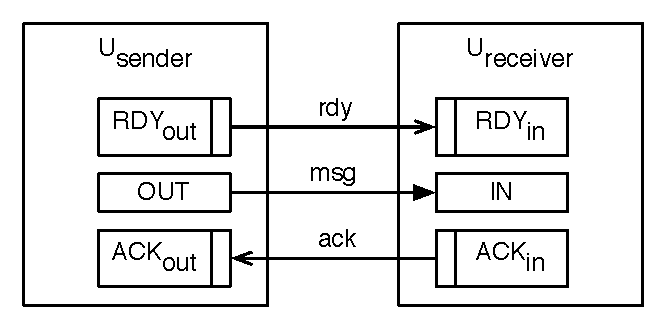
\includegraphics{firmware_communication.pdf}}
    \caption{Comunicazione simmetrica}
    \label{fig:fwcomm_sym}
  \end{subfigure}
  \begin{subfigure}[b]{.5\textwidth}
    \centering
    \resizebox{.8\columnwidth}{!}{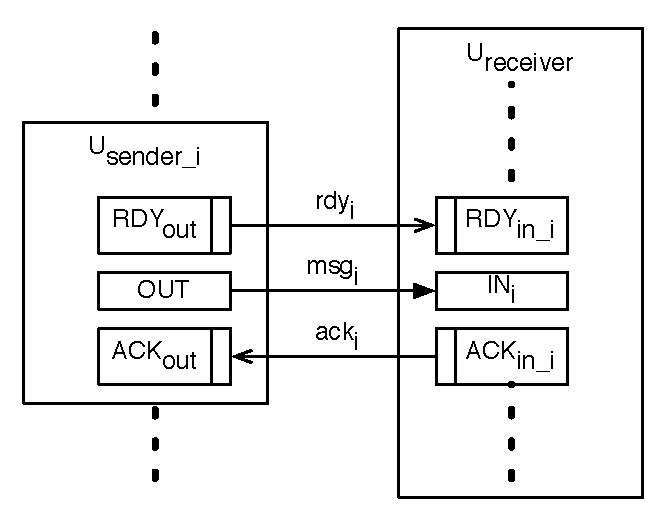
\includegraphics{firmware_asym_comm.pdf}}
    \caption{Comunicazione asimmetrica}
    \label{fig:fwcomm_asym}
  \end{subfigure}
  \caption{Componenti di un canale di comunicazione firmware}
  \label{fig:fwcomm}
\end{figure}

Si consideri la comunicazione simmetrica, il protocollo definisce due eventi: ``la presenza di un messaggio nel canale'' e ``la ricezione del messaggio da parte del ricevente''; nel livello firmware tali eventi sono realizzati tramite due collegamenti di un bit detti di Ready (Rdy) e di Acknowledgement (Ack) e da una coppia di indicatori di interfaccia per ciascun collegamento. Un canale di comunicazione a livello firmware \`e perci\`o costituito da tre componenti: l'interfaccia di uscita, il collegamento fisico e l'interfaccia di ingresso. Le interfacce contengono l'indicatore di uscita, quello di ingresso e il registro di uscita contenente il dato da trasmettere. Il collegamento \`e costituito dalle linee per connettere gli indicatori e i registri delle due interfacce. Un indicatore di interfaccia di uscita mette a disposizione l'operazione \emph{set} che provoca l'assunzione del valore 1 nell'indicatore di interfaccia di ingresso ad esso collegato. Un indicatore di interfaccia di ingresso mette a disposizione l'operazione \emph{test} con la quale viene letto il valore dell'indicatore, e l'operazione \emph{reset} con l'esecuzione della quale viene impostato a 0 il valore di uscita dell'indicatore stesso. Considerando due unit\`a $\mathrm{U}_{\mathrm{sender}}$ e $\mathrm{U}_{\mathrm{receiver}}$ collegate dai collegamenti \emph{rdy(1)}, \emph{msg(L)}, \emph{ack(1)} come in figura \ref{fig:fwcomm_sym}, il protocollo di comunicazione \`e perci\`o definito come in codice~\ref{lst:sym_firmware}
\begin{lstlisting}[language={}, morekeywords={msg, vtg}, float=t, caption={Descrizione astratta del protocollo di comunicazione del canale firmware simmetrico}, label={lst:sym_firmware}]
$\mathtt{U}_{\mathtt{sender}}$:send ::
  wait until $\mathtt{ACK}_{\mathtt{out}}$.test() is equal to 1
  send message msg to receiver and
    do $\mathtt{RDY}_{\mathtt{out}}$.set() and 
    do $\mathtt{ACK}_{\mathtt{out}}$.reset()

$\mathtt{U}_{\mathtt{receiver}}$:receive ::
  wait until $\mathtt{ACK}_{\mathtt{in}}$.test() is equal to 1
  use msg received and 
    do $\mathtt{ACK}_{\mathtt{in}}$.set() and
    do $\mathtt{RDY}_{\mathtt{in}}$.reset()
\end{lstlisting}

Il protocollo di comunicazione del canale asimmetrico in ingresso segue da quello descritto nel caso simmetrico: dal punto di vista logico \`e come se venissero adottati tanti canali simmetrici quante sono le unit\`a mittenti, ogni canale collega una unit\`a mittente all'unit\`a destinataria, figura \ref{fig:fwcomm_asym}. Il comportamento della funzione di invio rimane invariato rispetto a quello descritto precedentemente. Quello della funzione di ricezione testa tutti gli indicatori di tipo Rdy e con una certa politica ne seleziona uno tra quelli attivi ed esegue il protocollo del caso simmetrico, leggendo il valore, resettando il Rdy e inviando l'ack per il canale scelto.


\newpage
\subsection{Specifica dei canali di comunicazione}
\label{sct:specif_meccanismi_intro}
\begin{figure}[!t]
  \begin{subfigure}[b]{.5\textwidth}
    \centering
    %% \resizebox{\columnwidth}{!}{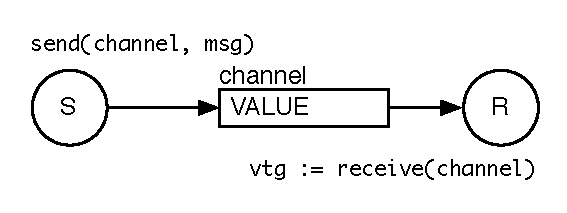
\includegraphics{abstract_sym.pdf}}
    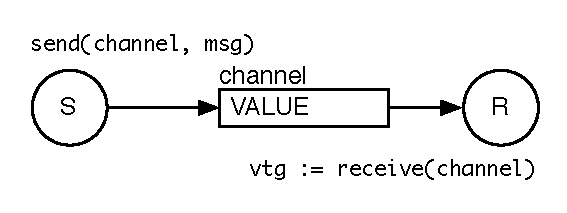
\includegraphics[scale=.5]{abstract_sym.pdf}
    \caption{Canale simmetrico}
    \label{fig:abstract_channel_sym}
  \end{subfigure}
  \begin{subfigure}[b]{.5\textwidth}
    \centering
    %% \resizebox{\columnwidth}{!}{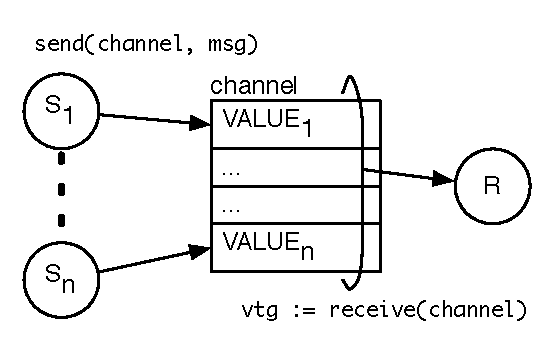
\includegraphics{abstract_asym.pdf}}
    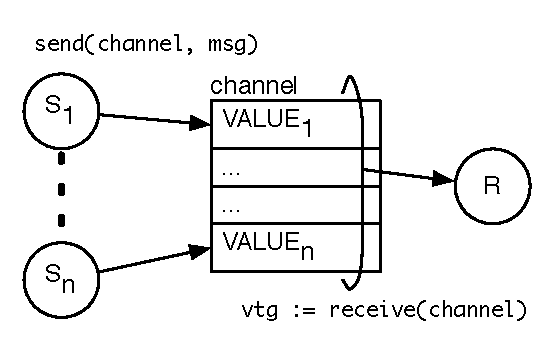
\includegraphics[scale=.5]{abstract_asym.pdf}
    \caption{Canale asimmetrico in ingresso}
    \label{fig:abstract_channel_asym}
  \end{subfigure}
  \caption[Canali di comunicazione tra processi]{Rappresentazione astratta di canali con grado di asincronia unitario}
  \label{fig:abstract_channels}
\end{figure}

%% >>>> INTRODUZIONE
%% ---> TODO
%% Si desidera implementare meccanismi di \emph{fast} message passing, in particolare canali di comunicazione simmetrici e asimmetrici in ingresso con grado di asincronia 1 e tipo di dato ``riferimento''. Si applica la copia del valore del messaggio nel canale.

%%Al fine di poter offrire un supporto efficiente ai paradigmi di programmi paralleli caratterizzati da grana fine sia nelle computazioni nei processi che nelle comunicazioni tra processi \`e stata studiata l'implementazione di meccanismi di \emph{fast} message passing nel CMP \tile. Meccanismi di questo tipo sono caratterizzati da una bassa latenza di comunicazione, 

%% Le forme di comunicazione che sono espresse da tali meccanismi sono sufficienti per fornire il supporto dei principali paradigmi di programmazione parallela. Il grado di asincronia unitario risulta sufficiente per le forme di parallelismo e consente minori overhead nell'implementazione dei meccanismi rispetto a gradi di asincronia maggiori di uno.

%% >>>> DESCRIZIONE DEI MECCANISMI
Con canale di comunicazione si intende il collegamento logico tramite il quale due o pi\`u processi comunicano. L'astrazione di canale come meccanismo primitivo di scambio di informazioni tra processi viene fornita dal supporto a tempo di esecuzione della nostra libreria. Il canale \emph{simmetrico} \`e un oggetto che mette in comunicazione un processo mittente con un processo destinatario, consentendo l'invio di messaggi dal processo mittente al processo destinatario. Un canale \emph{asimmetrico in ingresso} \`e un oggetto che mette in comunicazione pi\`u processi mittenti con un singolo processo destinatario, consentendo a ciascun mittente l'invio di messaggi al processo destinatario. Il destinatario riceve i messaggi in modo non deterministico e senza saperne la provenienza, a meno di comunicazioni esplicite. 

Per entrambi i canali sono definite due primitive di comunicazione, quella di invio e quella di ricezione le quali sono usate rispettivamente dal processo mittente e dal processo destinatario del canale di comunicazione. Si considera la seguente dichiarazione C delle primitive:
\begin{lstlisting}[morekeywords={ch_sym_t, ch_asym_t}]
void sym_send(ch_sym_t *ch_descr, const void *msg)
void *sym_receive(ch_sym_t *ch_descr)

void asym_send(ch_asym_t *ch_descr, const void *msg, int rank)
void *asym_receive(ch_asym_t *ch_descr)
\end{lstlisting}
Ad ogni primitiva viene quindi passato, come primo parametro, il descrittore di canale come riferimento ad una struttura dati allocata in memoria condivisa. Non viene usata la tecnica zero-copy in quanto non \`e applicabile all'implementazione che fa uso della UDN. La primitiva di invio ha come secondo parametro il valore del messaggio, quella di ricezione ritorna il valore letto dal canale come valore di ritorno, il valore del messaggio \`e copiato prima nel canale poi nella variabile targa. Nel caso asimmetrico \`e necessario specificare alla primitiva di invio l'identificatore del mittente all'interno del canale, ci\`o \`e necessario per l'implementazione, come spiegato nelle sezioni successive per entrambi i supporti.

%% >>>> SPECIFICA PRIMITIVE DI COMUNICAZIONE
Si considera il seguente comportamento ad alto livello delle due forme di comunicazione con il grado di asincronia considerato:
%% Si considerano le seguenti specifiche del comportamento della primitiva di invio su un canale simmetrico con grado di asincronia unitario:
\begin{description}
\item [canale simmetrico con grado di asincronia unitario] prevede che il processo mittente possa inviare fino ad un messaggio senza attendere che il destinatario lo abbia ricevuto. Nel caso in cui il mittente intenda inviare un secondo messaggio senza che il destinatario abbia ricevuto quello precedente occorre che il mittente attenda la ricezione da parte del destinatario.
\item [canale asimmetrico in ingresso con grado di asincronia unitario] \hfill ogni processo mittente pu\`o inviare fino ad un messaggio senza attendere che il destinatario lo abbia ricevuto. Nel caso in cui un generico mittente intenda inviare un secondo messaggio senza che il destinatario abbia ricevuto il messaggio precedentemente inviato dal quello specifico mittente, occorre che tale mittente attenda la ricezione da parte del destinatario del messaggio precedente. 
\end{description}
Per quanto riguarda il comportamento del ricevente di un canale asimmetrico, non si impone una specifica politica di ricezione. Il comportamento che pu\`o essere considerato naturale \`e la ricezione FIFO dei messaggi inviati dai mittenti, tuttavia tale funzionamento non \`e imposto. Si pu\`o infatti parlare del canale asimmetrico in ingresso come un caso particolare di comportamento non deterministico del destinatario nella ricezione da pi\`u canali simmetrici.

\begin{lstlisting}[
    float = b,
    caption = {Descrizione astratta del protocollo di comunicazione per un canale simmetrico con grado di asincronia 1}, 
    label = lst:abstract_sym_protocol,
    morekeywords={msg, vtg, ready, acknowledgement, sender, receiver}
]
send ::
  wait until acknowledgement signal is received
  send the message to receiver and
    reset acknowledgement flag and
    signal ready to the receiver
  
receive ::
  wait until ready signal is received
  copy the message received from sender into vtg and
    reset ready flag and
    signal acknowledgement to the sender
\end{lstlisting}
Nelle sezioni successive verranno descritte le implementazioni dei due tipi di canale che sfruttano supporti architetturali diversi. I protocolli di comunicazione che costituiscono l'implementazione con i diversi supporti fanno riferimento al protocollo usato al livello firmware per la comunicazione di due unit\`a di elaborazione indipendente dal tempo. Tale protocollo \`e chiamato nel seguito Rdy-Ack. Descriviamo qui, in modo astratto, le azioni dei processi comunicanti definite dal protocollo che assicurano la correttezza della comunicazione, ovvero: 
\begin{itemize}
\item non si verifica mai la perdita di un messaggio,
\item se il/un processo mittente invia un messaggio allora prima o poi il processo destinatario lo deve ricevere,
\item se il processo destinatario riceve un messaggio allora prima o poi il processo mittente che ha effettuato l'invio di quel messaggio deve essere in grado di inviarne un altro.
\end{itemize}
%% >>>> DESCRIZIONE DEL PROTOCOLLO
Per il canale simmetrico si hanno le azioni delle due entit\`a descritte nel codice~\ref{lst:abstract_sym_protocol}. Il canale asimmetrico in ingresso ha protocollo simile, in quanto pu\`o essere visto come costituito da tanti canali simmetrici Rdy-Ack quanti sono i mittenti, dove ogni canale collega un mittente al destinatario. Il comportamento dell'invio di un messaggio \`e esattamente lo stesso di quello adottato nel canale simmetrico, mentre la ricezione ha l'onere di scegliere in modo non deterministico un canale da cui ricevere tra i canali pronti.



%% che il \emph{mapping} delle applicazioni parallele considerate nell'architettura \`e di \emph{tipo esclusivo}, ovvero esiste una corrispondenza biunivoca tra ogni processo dell'applicazione e il processore della macchina che lo esegue. 
%% ---> MOTIVAZIONI

\newpage
\FloatBarrier
\subsection{Implementazione dei canali con memoria condivisa}
\label{sct:specifica_sm}
Sfruttando la memoria condivisa si ha una implementazione semplice e lock-free delle comunicazioni simmetrica e asimmetrica con il protocollo Rdy-Ack. Ci\`o \`e determinato dal fatto che non esiste un buffer o altre strutture dati sulle quali i processi devono accedere in modo indivisibile. L'adozione di un grado di asincronia unitario e la sincronizzazione tramite gli eventi Rdy e Ack permette di effettuare accessi al descrittore del canale senza la necessit\`a di mutua esclusione.

\subsubsection{Comunicazione simmetrica}
\label{sct:sym_sm_rdyack}
Si considera la comunicazione simmetrica: il descrittore di canale \`e costituito da tre informazioni:
\begin{inparaenum}[\itshape a~\upshape)] 
\item il valore di Rdy, \item il valore di Ack, \item il valore del messaggio.
\end{inparaenum}
Ogni informazione \`e allocata in una parola, in particolare abbiamo la seguente definizione del descrittore di canale:  i flag di Rdy e di Ack sono di tipo intero, il messaggio \`e di tipo riferimento.
\begin{lstlisting}
struct ch_sym_sm_rdyack_t { 
  int rdy; 
  int ack; 
  void *value;
};
\end{lstlisting}
La segnalazione di un evento di Rdy o di Ack avviene impostando al valore 1 il corrispondente campo nel descrittore di canale. L'attesa attiva di un processo sul canale \`e realizza con la strategia \emph{retry} sul valore del flag Rdy o Ack: si continua a testare il valore del flag fino a quando non assume valore 1.
Il protocollo di comunicazione viene perci\`o realizzato con le seguenti azioni:
\begin{lstlisting}[
        morekeywords={rdy, ack, value},
        caption={Descrizione astratta del protocollo di comunicazione Rdy-Ack su memoria condivisa},
        label={lst:abstr_mem_sym}
]       
send(ch_descr, msg) ::
  wait until ch_descr->ack flag is equal to 1;
  reset ch_descr->ack flag to 0;
  copy msg into ch_descr->value entry;
  memory_fence();
  set ch_descr->rdy flag to 1;

receive(ch_descr) ::
  wait until ch_descr->rdy flag is equal to 1;
  reset ch_descr->rdy flag to 0;
  read the ch_decsr->value entry;
  set ch_descr->ack flag to 1;
\end{lstlisting}
La mutua esclusione nell'uso del valore del canale da parte dei processi mittente e destinatario \`e garantita dalla sincronizzazione dei due processi sui due valori di Rdy e Ack: ogni processo accede al valore del canale solo dopo che il processo partner ha notificato tale possibilit\`a. Per garantire la correttezza della comunicazione \`e quindi sufficiente adottare la seguente condizione iniziale:
\begin{itemize}
\item all'avvio dell'applicazione tutti i canali devono avere descrittore con campo Ack inizializzato ad 1 e capo Rdy inizializzato a 0.
\end{itemize}
Tale condizione iniziale, insieme all'adozione del protocollo, garantisce la seguente propriet\`a:
\begin{itemize}
\item ogni notifica di evento Rdy o Ack trova sempre l'evento corrispondente precedentemente falso.
\end{itemize}

%% L'IMPLEMENTAZIONE \`E LOCK-FREE, NECESSARIA MEMORY FENCE
Il fatto che sia possibile evitare l'uso di meccanismi di lock per l'esecuzione indivisibile del codice \`e un aspetto positivo dell'implementazione con memoria condivisa del protocollo Rdy-Ack, in quanto si evitano i relativi overhead sulle prestazioni. Al fine di garantire la correttezza \`e tuttavia richiesto l'uso di scritture sincrone alla memoria condivisa. \`E necessario che le scritture effettuate dal mittente sul valore del canale e sul flag di Rdy siano viste dal destinatario nello stesso ordine. Come descritto in sezione~\ref{sct:intro_arch_memory}, \tile\ adotta un modello rilassato di consistenza della memoria, sia per quanto riguarda l'ordinamento di istruzioni all'interno di una CPU, sia per l'atomicit\`a delle scritture in memoria condivisa. Ci\`o rende necessario l'uso di una barriera di memoria tra le due scritture effettuate dal mittente (riga 5 del codice~\ref{lst:abstr_mem_sym}), in modo che la scrittura del valore 1 sul flag Rdy sia sempre vista dal processo destinatario dopo la scrittura del messaggio nel canale. Il comportamento sincrono delle scritture in memoria, indotto dall'uso della barriera, produce overheads aggiuntivi rispetto al comportamento asincrono delle scritture. La barriera della memoria, e la corrispondente degradazione delle prestazioni, pu\`o essere eliminata con l'adozione di un protocollo di comunicazione alternativo, come mostrato in sezione~\ref{sct:sym_sm_nullack}.

%% USO SEMPRE LA CACHE
La politica di attesa attiva \emph{retry} \`e caratterizzata da un aumento dei conflitti alla memoria principale. Per evitare ci\`o e ridurre la latenza di sveglia si prendono in considerazione solo implementazioni che fanno uso della gerarchia cache. In tale scenario la prima lettura del valore di un flag causa il trasferimento del blocco corrispondente nei livelli L2 e L1D della cache locale, e le letture successive del valore del flag rimangano interne alla CPU, in quanto servite dalla cache locale. Quando il processo partner esegue la scrittura sul flag il meccanismo di coerenza della cache provvede a notificare il cambiamento e aggiornare il valore nella cache locale.

%% EFFETTO SULLE PRESTAZIONI DELLA COERENZA CACHE
Come descritto in sezione~\ref{sct:intro_arch_cache} il meccanismo di coerenza della cache \`e configurabile in molti aspetti, in particolare \`e possibile impostare il PE Home per una certa pagina di memoria. 
In sezione~\ref{sct:intro_arch_cache} viene spiegato come l'uso della strategia \emph{Remote Homing} sia conveniente in computazioni con singolo consumatore di una struttura dati condivisa, e permetta di evitare l'uso di invalidazioni e conseguenti copie di blocchi.
%, consentendo invece l'attuazione di un modello di programmazione di tipo \emph{remote storing}. 
Di seguito descriviamo il comportamento della comunicazione simmetrica con il protocollo Rdy-Ack e il descrittore di canale presentati, con la configurazione predefinita della coerenza della cache, quindi verr\`a presentata una versione ottimizzata che minimizza i messaggi di coerenza e le copie dei blocchi grazie alla configurazione dei PEs Home e al partizionamento del descrittore del canale nelle cache dei PEs.

%% USO PREDEFINITO DELLA COERENZA CACHE
\begin{figure}[!t]
  \centering
  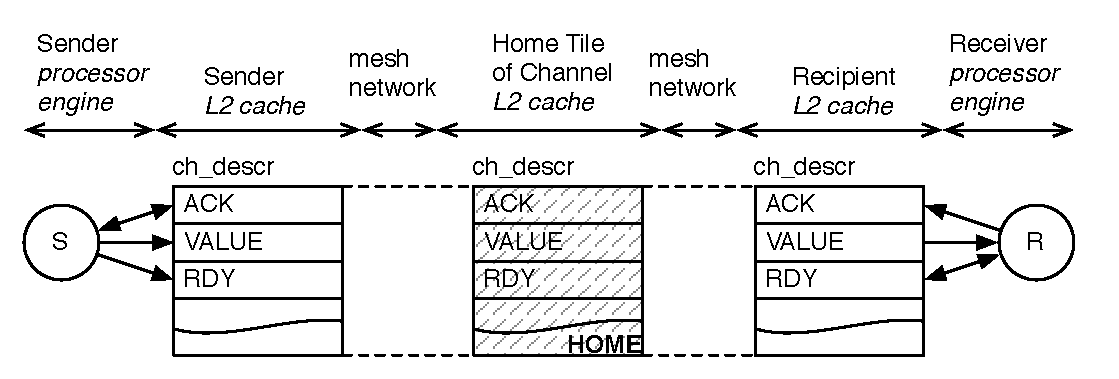
\includegraphics[scale=.5]{cache_sym_sm_no.pdf}
  \caption[Comunicazione simmetrica su memoria condivisa, non ottimizzata]{Rappresentazione di una comunicazione simmetrica tra un processo mittente $S$ e uno destinatario $R$ con uso della memoria condivisa e gestione predefinita della coerenza di cache (hash-for-home strategy)} 
  \label{fig:cache_sym_sm_no}
\end{figure}
La strategia predefinita di allocazione delle pagine di memoria nelle cache \`e \emph{Hash-for-Home} \cite{ug205}. La gestione delle informazioni di coerenza di cache, in particolare l'entrata della Directory, del blocco che contiene il descrittore di canale allocato viene affidata ad un generico processing element $\mathrm{PE}_k$. Durante l'esecuzione del programma parallelo il processo mittente, eseguito in $\mathrm{PE}_i$, e il processo destinatario, eseguito in $\mathrm{PE}_j$, eseguono, per mezzo delle primitive di comunicazione, degli accessi al descrittore di canale. In generale $k \neq i$ e $k \neq j$ quindi si hanno tre copie del blocco contenente il descrittore di canale come mostrato in figura~\ref{fig:cache_sym_sm_no}. La modifica di un campo del descrittore del canale effettuata da uno dei due processi comunicanti provoca l'invalidazione del blocco di L2 nel PE che esegue il processo partner. Quando il PE che contiene il blocco invalidato riferisce il descrittore di canale, l'intero blocco sar\`a trasferito dal PE Home, $\mathrm{PE}_k$, al PE stesso. Nel caso migliore si ha una invalidazione e corrispondente trasferimento di blocco al termine di ogni esecuzione di una primitiva di comunicazione, quando viene notificato un evento di sincronizzazione al processo partner per mezzo di una scrittura nel descrittore di canale.
%% USO OTTIMIZZATO DELLA COERENZA CACHE
\begin{table}[!b]
  \begin{center}
    \begin{tabular}{ | l | l | l | l |}
      \hline
      & Rdy & Ack & Value \\ \hline
      Sender & Write Only & Read and Write & Write Only \\
      Receiver & Read and Write & Write Only & Read Only \\
      \hline
    \end{tabular}
  \end{center}
  \caption[Modalit\`a di accesso ad un canale su memoria condivisa]{Modalit\`a di accesso ai campi del descrittore di canale su memoria condivisa}
  \label{tab:accessi_descr_ch}
\end{table}

Questo offre lo spunto su come ottimizzare l'uso delle cache: la scrittura sul campo del descrittore di canale che implementa un segnale di sincronizzazione dovrebbe essere inoltrata direttamente alla cache del PE che attende il segnale, evitando il trasferimento di un blocco di L2 per la trasmissione di una sola parola. 
%Tale comportamento \`e simile al modello di Remote Store Programming nel quale un processo pu\`o scrivere nella memoria locale di un altro processo.
Questo comportamento \`e possibile in quanto:
\begin{itemize}
\item per ogni campo del descrittore esiste uno solo dei due processi che vi accede in lettura(vedi tabella~\ref{tab:accessi_descr_ch}),
\item \`e possibile impostare il PE Home di un certo blocco di cache L2,
\item come descritto nella sezione~\ref{sct:intro_arch_cache} un PE che \`e Home per un blocco detiene sempre la copia corretta del blocco stesso.
\end{itemize}
%Dato che per ciascun campo del descrittore di canale esiste un unico consumatore (vedi tabella~\ref{tab:accessi_descr_ch}),  \`e possibile applicare alle cache L2 il modello RSP utilizzando la strategia di allocazione Remote Homing del \tile. 
%% Partizionando opportunamente il descrittore di canale e configurando come PE Home quei core nel quale viene eseguito il processo che consuma tali dati, abbiamo come risultato che le scritture a tali dati sono dirette e locali al PE che \`e consumatore dei dati.
Il descrittore di canale viene partizionato in due parti, allocate in blocchi distinti e con diverse configurazioni di Homing:
%\begin{inparaenum}[\itshape1\upshape)] 
\begin{description}
\item [la parte di output] contiene tutti i campi acceduti in lettura del mittente (Ack), ed \`e allocata impostando come PE Home quello che esegue il processo mittente, 
\item [la parte di input] contiene tutti i campi acceduti in lettura dal mittente (Rdy e Value), ed \`e allocata impostando come PE Home quello che esegue il processo destinatario.
\end{description}

Con tale configurazione si incrementa la localit\`a delle informazioni: la coerenza dei dati e l'allocazione degli stessi avviene nella cache del PE che consuma tali dati, permettendo al PE produttore di effettuare scritture direttamente nella cache locale del consumatore tramite messaggi write-through. I processo consumatore dei dati trova le informazioni gi\`a aggiornate direttamente nella cache locale alla CPU che lo esegue. 

Si osserva inoltre che, in tale computazione, il processo consumatore di una informazione esegue anche scritture sul blocco, ci\`o causa l'invio di messaggi di invalidazione del blocco alla cache L2 del PE che esegue il produttore. Tuttavia in futuro non si verificher\`a mai un trasferimento del blocco in quanto il produttore esegue \emph{esclusivamente} scritture sul blocco, ci\`o causa l'allocazione del blocco nella L2 locale (quando il blocco \`e non valido), la modifica della singola parola scritta e l'invio del messaggio Write-Through alla cache L2 del PE consumatore.
\FloatBarrier
\begin{figure}[!t]
  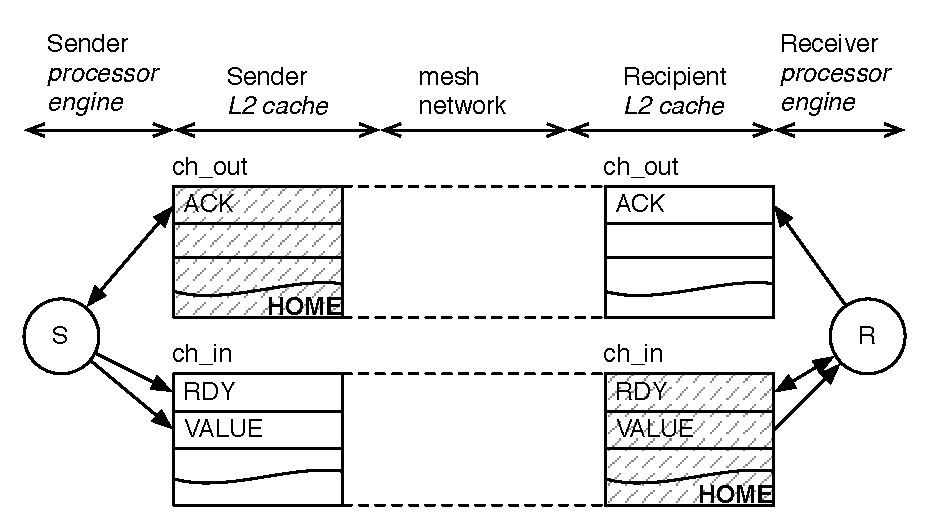
\includegraphics[scale=.5]{cache_sym_sm_fence.pdf}
  \centering
  \caption[Comunicazione simmetrica su memoria condivisa]{Rappresentazione di una comunicazione simmetrica tra i processi $S$ e $R$ con uso della memoria condivisa e gestione ottimizzata della coerenza di cache con strategia Remote Homing per il descrittore di canale}
  \label{fig:cache_sym_sm_fence}
\end{figure}

In conclusione si fa presente che esiste un terzo blocco di cache, usato per il supporto del canale di comunicazione, che contiene i riferimenti alle due parti del descrittore di canale. Tale blocco \`e sempre acceduto in sola lettura, quindi non presenta particolari problemi per le prestazioni e pu\`o essere allocato in uno dei due PE comunicanti con strategia Remote Homing oppure in un terzo PE con strategia Hash-for-Home.

\newpage

\FloatBarrier
\subsubsection{Comunicazione asimmetrica in ingresso}
\label{sct:asymin_sm_rdyack}
Il canale asimmetrico in ingresso \`e visto come costituito da tanti canali simmetrici quanti sono i mittenti. Al fine di ottimizzare le prestazioni non si usa direttamente l'implementazione del canale simmetrico ma si sfruttano comunque i risultati e l'analisi di tale meccanismo, in particolare per quanto riguarda l'allocazione degli oggetti condivisi in cache al fine di garantire la maggiore localit\`a possibile. 

Siano $n$ i processi mittenti del canale, dal punto di vista logico il canale asimmetrico usa $n$ canali simmetrici implementati con il protocollo Rdy-Ack, e perci\`o caratterizzati dal valore della tripla $<Rdy,\; value,\; Ack>$. Come descritto nella sezione \ref{sct:sym_sm_rdyack} i valori di  $Rdy$ e $value$ di un canale simmetrico sono allocati in un blocco che ha per Home il PE che esegue il ricevente mentre $Ack$ ha per Home il il PE che esegue il mittente. Per minimizzare il numero dei blocchi allocati in cache si raggruppa l'insieme dei Rdy e dei valori $\{ <Rdy_i,\; value_i> |\; i \in \{ 1, \dots, n\} \}$ allocandolo come vettore di $n$ coppie $<Rdy,\;value>$ e impostando come Home il PE destinatario, con strategia Remote Homing. I valori di $Ack$ sono invece allocati ciascuno in un blocco che ha per home il PE mittente corrispondente, questo consente la maggior localit\`a possibile. 

Si fa presente che sebbene tale configurazione permetta la massima localit\`a delle informazioni ai PEs, presenta tuttavia l'allocazione nella cache L2 del destinatario di un numero di blocchi che \`e lineare rispetto al numero dei mittenti: si hanno $\frac{2 \cdot 4 \cdot n}{64}$ blocchi necessari a memorizzare l'array di coppie $<Rdy,\;value>$ e $n$ blocchi allocati per le scritture sui flag $Ack$ degli $n$ mittenti. Considerando il caso della comunicazione con il massimo numero (63) di mittenti, si hanno 72 blocchi allocati nel PE destinatario, ovvero uno spazio di 4.5 KB su un totale di 64KB nella cache L2. Dato che siamo interessati a massimizzare le prestazioni si assume che l'uso di tale spazio nella L2 del destinatario non sia problematico per l'applicazione. 

Si osserva che, soprattutto con un numero elevato di mittenti, la sveglia del destinatario sar\`a pi\`u lenta rispetto a quella nel canale simmetrico, infatti l'attesa \`e implementata eseguendo la scansione delle variabili $Rdy$ perci\`o nel caso peggiore \`e necessario effettuare $n$ accessi alla memoria dalla scrittura del valore 1 in un flag $Rdy$ da parte del mittente.

Il descrittore di canale \`e costituito da $n$ riferimenti ai valori di $Ack$ allocati con strategia Remote Homing nei PEs mittenti, e il riferimento alla base del vettore delle coppie $<Rdy, value>$ allocato con strategia Remote Homing nel PE destinatario. Come descritto nella sezione~\ref{sct:specif_meccanismi_intro} il protocollo di comunicazione rimane sosta\-nzialmente invariato rispetto al caso simmetrico, rimane da specificare la politica adottata dal ricevente per selezionare il mittente da cui ricevere tra quelli che hanno inviato un nuovo messaggio. Il supporto della primitiva di ricezione adotta una scansione lineare dell'insieme dei flag $Rdy$ alla ricerca di uno attivo. Ad ogni ricezione viene salvato l'indice del mittente da cui si \`e effettuata la lettura, in modo tale che alla prossima esecuzione della ricezione la scansione dei $Rdy$ si avviata dal mittente successivo. La ricezione \`e quindi non deterministica ed \`e attuata un politica di fairness, sebbene la propriet\`a non sia formalmente soddisfatta. 

Al fine di attuare il protocollo di comunicazione esiste una questione che l'implementazione del supporto della primitiva di invio deve risolvere: conoscere l'identificatore all'interno del canale asimmetrico del mittente che ha eseguito la primitiva. Tale informazione \`e ovviamente indispensabile al protocollo di invio, tra le possibili soluzioni si sono valutate le seguenti due:
\begin{itemize}    
\item la primitiva di invio contiene un terzo parametro, l'identificatore del mittente nel canale, oltre al riferimento al descrittore di canale e al valore del messaggio,
\item ogni mittente usa un proprio descrittore di canale che contiene l'identificatore all'interno del canale, per far ci\`o \`e necessaria una funzione di inizializzazione eseguite da ogni mittente prima dell'avvio della computazione.
\end{itemize}
Si \`e scelta la prima soluzione in quanto anche l'implementazione che sfrutta la UDN verifica lo stesso problema perci\`o \`e assicurata l'uniformit\`a della primitiva di invio nelle due implementazioni del canale asimmetrico. \`E responsabilit\`a dell'utente far si che ogni processo mittente del canale conosca il proprio identificatore univoco all'interno del canale e quindi poter invocare correttamente la primitiva di invio sul canale.
%% 2 * 4 * 64 / 64 + 64 = 8 + 64 = 72 blocchi = 72 * 64 B = 4608 B = 4.5 KB = 1152 word su un totale di 64KB
\begin{figure}[!tb]
  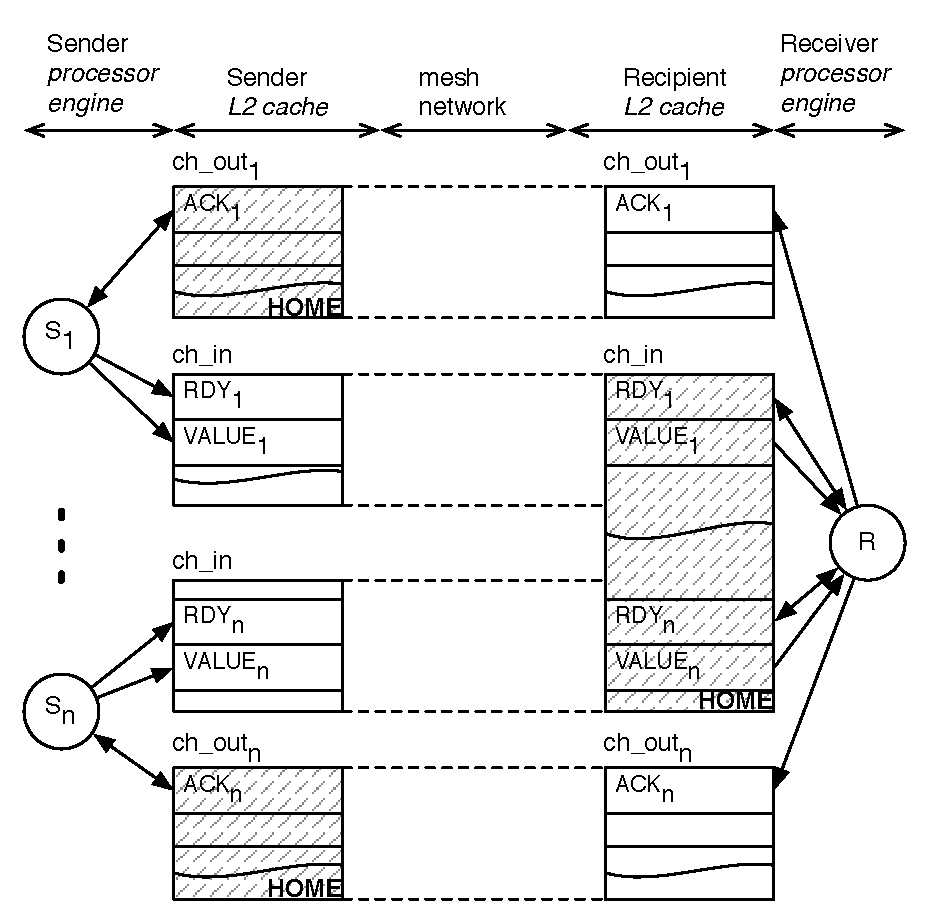
\includegraphics[scale=.5]{cache_asym_sm.pdf}
  \centering
  \caption[Comunicazione asimmetrica su memoria condivisa]{Rappresentazione di una comunicazione asimmetrica tra i processi $\{S_1, \ldots, S_n\}$ e $R$ con uso della memoria condivisa e gestione ottimizzata della coerenza di cache con strategia Remote Homing per il descrittore di canale}
  \label{fig:cache_asym_sm}
\end{figure}

\FloatBarrier
\subsubsection{Comunicazione simmetrica senza barriera di memoria}
\label{sct:sym_sm_nullack}
Nella sezione~\ref{sct:sym_sm_rdyack} si \`e descritta l'implementazione del supporto alla comunicazione simmetrica per mezzo di strutture dati lock-free e, per garantire la correttezza, l'uso della barriera di memoria nel supporto della primitiva di invio. Si propone un'altra possibile implementazione della comunicazione simmetrica con un diverso protocollo che consente il corretto funzionamento con strutture dati lock-free senza l'uso di barriere di memoria. Il protocollo che si va a definire si rif\`a a quello Rdy-Ack, in quanto sono mantenuti gli eventi di sincronizzazione ``messaggio pronto'' (Rdy) e ``messaggio ricevuto'' (Ack). In questo caso l'evento di Rdy non \`e segnalato esplicitamente ma risulta implicito nel cambiamento di valore del canale. Viene infatti definito il valore particolare $\alpha$ che non pu\`o essere assunto dai messaggi trasmessi nel canale e che indica la situazione in cui il canale \`e vuoto. 
Il canale assume valore $\alpha$ all'avvio dell'applicazione e al termine di ogni esecuzione della primitiva di ricezione.
Il flag \verb+Rdy+ \`e eliminato dall'implementazione, il destinatario usa il valore del canale e il valore $\alpha$ per determinare la presenza di un nuovo messaggio, come descritto in codice~\ref{lst:abstr_mem_sym_nullack}. 

Anzitutto si osserva che tale protocollo si applica bene alla nostra implementazione dei canali, in quanto si pu\`o definire, senza perdere di generalit\`a, il valore particolare $\alpha$ come il valore di puntatore ``nullo'': \verb+NULL = (void *) 0+. 
Passando all'analisi della correttezza, la barriera di memoria \`e stata eliminata nella primitiva di invio, in quanto esiste un unico oggetto (il campo \verb+value+) che \`e scritto dal mittente ed \`e acceduto da altri processi.
Nella primitiva di ricezione si hanno invece due oggetti, i campi \verb+value+ e \verb+ack+, che sono scritti dal ricevente ed acceduti dal processo partner. Grazie alla specifica politica di homing di tali oggetti e alla modalit\`a di accesso a questi del processo mittente, l'uso di una memory fence non \`e necessario. Risulta invece sufficiente che il PE che esegue il processo destinatario produca le due scritture nell'ordine specificato. Il campo \verb+value+ ha per Home il PE che esegue il processo ricevente ed \`e acceduto in scrittura dal processo mittente dopo aver letto la variazione di valore del campo \verb+ack+. La prima scrittura \`e quindi locale alla L2 del ricevente, inoltre non ha importanza in che istante diventa visibile agli altri PEs, in quanto l'oggetto scritto (\verb+value+) \`e acceduto in sola scrittura dal mittente. La seconda scrittura \`e una write-through alla L2 del mittente, il quale, una volta letto il nuovo valore pu\`o effettuare una nuova scrittura sul campo \verb+value+ che sicuramente \`e gi\`a stato modificato a \verb+NULL+. Per imporre l'ordinamento delle istruzioni nel PE ricevente si usa l'istruzione \verb+compiler_barrier()+, la quale \`e molto diversa da una barriera di memoria. Il comportamento delle scritture infatti resta asincrono, si \`e solo negato lo spostamento di codice da parte del compilatore, e quindi un ordine diverso di produzione delle due scritture.

\begin{lstlisting}[
        float=t,
        morekeywords={ack, value}, 
        caption={Descrizione astratta del protocollo di comunicazione Null-Ack su memoria condivisa},
        label={lst:abstr_mem_sym_nullack}
]
send(ch_descr, msg) ::
  wait until ch_descr->ack flag is equal to 1;
  reset ch_descr->ack flag to 0;
  copy msg into ch_descr->value entry;

receive(ch_descr) ::
  wait until ch_descr->value is not equal to NULL;
  read the ch_descr->value entry;
  set ch_descr->value to NULL;
  compiler_barrier();
  set ch_descr->ack flag to 1;
\end{lstlisting}

\newpage
\FloatBarrier
\subsection{Implementazione dei canali con UDN}
\label{sct:specifica_udn}
L'uso della UDN permette sia la sincronizzazione dei processi che la trasmissione dei dati tra processi, con latenze molto basse e senza l'utilizzo della memoria condivisa e quindi del sottosistema di cache. A tal fine \`e possibile pensare ad una associazione tra uno o pi\`u canali firmware UDN e un canale software. Esistono per\`o alcune limitazioni imposte da tale rete: 
\begin{itemize}
\item sono disponibili quattro canali UDN (fisici), ciascuno dei quali \`e associato univocamente ad una coda firmware nella CPU, utilizzata in lettura;
\item \`e fissata la massima dimensione dei pacchetti trasmessi nella rete, la quale non pu\`o superare la dimensione delle code firmware nelle CPU.
\end{itemize}
Ne segue che, volendo utilizzare solo la rete di interconnessione senza il supporto della memoria condivisa, il numero di canali software \`e limitato dal numero di canali firmware e che il grado di asincronia di un canale software possa essere limitato dalla dimensione delle code firmware. In altre parole non \`e possibile una implementazione dei canali di comunicazione tra processi che sfrutta esclusivamente UDN e che sia generica, non solo nel grado di asincronia, ma anche nel numero di canali disponibili per processo. Per ottenere tale genericit\`a \`e necessario far uso di memoria condivisa.
\FloatBarrier
\subsubsection{Comunicazione simmetrica}
\label{sct:sym_udn}
\begin{figure}[!b]
  \centering
  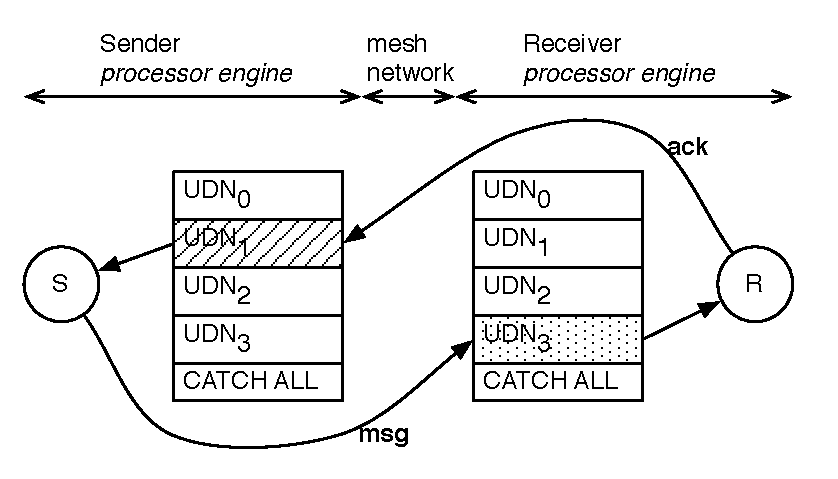
\includegraphics[scale=.5]{udn_sym.pdf}
  \caption[Comunicazione simmetrica su UDN]{Rappresentazione di un possibile scenario di comunicazione simmetrica tra il processo mittente S e quello destinatario R, sfruttando la UDN}
  \label{fig:udn_sym}
\end{figure}
Viene descritta l'implementazione della comunicazione simmetrica che sfrutta in modo ottimale la UDN. 
Tale implementazione pone alcuni limiti sull'utilizzo dei canali ma fornisce le migliori prestazioni possibli riguardo allo scambio dei messaggi sfruttando la UDN. Il protocollo Rdy-Ack per un canale simmetrico viene realizzato impiegando una coda UDN in entrambi i PE che eseguono i processi comunicanti. La coda firmware nel destinatario \`e usata per ricevere i messaggi, il segnale di Rdy \`e implicito con la ricezione di un nuovo messaggio, la coda firmware nel mittente \`e usata per i segnali di Ack, i quali sono esplicitati con l'invio di un messaggio di valore arbitrario di dimensione una parola dal destinatario a tale coda UDN nel mittente. Un possibile scenario \`e mostrato in figura~\ref{fig:udn_sym} dove il canale di comunicazione \`e implementato tramite l'utilizzo della seconda coda UDN nel processo mittente, per la ricezione dei segnali di Ack, e con la quarta coda UDN nel processo destinatario, per la ricezione dei messaggi; ne segue che in entrambi i PE, che eseguono esclusivamente il processo mittente o quello destinatario, rimangono disponibili altre tre code (o canali) UDN utilizzabili per altrettanti canali di comunicazione tra processi. Il protocollo di comunicazione segue quindi lo schema del codice~\ref{lst:abstr_udn_sym}: viene usata una struttura dati condivisa in memoria, il descrittore di canale, acceduta in sola lettura da entrambi i processi comunicanti, contenente l'identificatore delle cpu in cui i processi comunicanti sono eseguiti, e l'identificatore delle code UDN nei due PE, utilizzate dal canale per la comunicazione. La correttezza del protocollo si ottiene con due condizioni: \begin{inparaenum}[\itshape a~\upshape)] \item l'inizializzazione di un canale di comunicazione Rdy-Ack prevede l'invio del segnale di Ack al mittente all'avvio dell'applicazione, in questo caso deve essere inviata una parola arbitraria alla coda UDN usata nel canale dal processo mittente, \item un corretto uso da parte dell'utente dei canali nell'assegnazione delle code UDN a diversi canali di comunicazione: se un canale di comunicazione fa uso di una certa coda UDN, tale coda UDN non deve essere utilizzata da altri canali o da altri meccanismi.\end{inparaenum}
\begin{lstlisting}[
        float=t,
        morekeywords={dq_snd, dq_rcv, cpu_snd, cpu_rcv}, 
        caption={Descrizione astratta del protocollo di comunicazione Rdy-Ack su UDN per un canale di comunicazione simmetrico},
        label={lst:abstr_udn_sym}
]
send(ch_descr, msg) ::
  leggi una parola dalla UDN Demux Queue ch_descr->dq_snd
  invia tramite UDN il valore msg alla UDN Demux Queue 
    ch_descr->dq_rcv del PE ch_descr->cpu_rcv

receive(ch_descr) ::
  leggi una parola dalla UDN Demux Queue ch_descr->dq_rcv e
    assegna il valore alla variablie targa
  invia tramite UDN una parola arbitraria alla UDN Demux
    Queue ch_descr->dq_snd del PE ch_descr->cpu_snd
\end{lstlisting}

L'implementazione descritta limita perci\`o l'uso di questo tipo di canali ad un massimo di quattro canali per processo, l'implementazione bypassa completamente la memoria se non per accedere in sola lettura alle informazioni del canale, la trasmissione dei dati e la sincronizzazione dei processi/PE avviene a livello firmware grazie alla rete di interconnessione e alle primitive di accesso ad essa fornite dal sistema come letture e scritture su registri generali. 

Con il grado di asincronia unitario non esistono problemi di deadlock in quanto, se verificate le condizioni di correttezza, il protocollo garantisce la corretta sincronizzazione e i dati scambiati nella rete sono lunghi una sola parola, quindi non causano l'overrun delle code UDN.

\FloatBarrier
\subsubsection{Comunicazione asimmetrica in ingresso}
\label{sct:asym_udn}
\begin{figure}[!t]
  \centering
  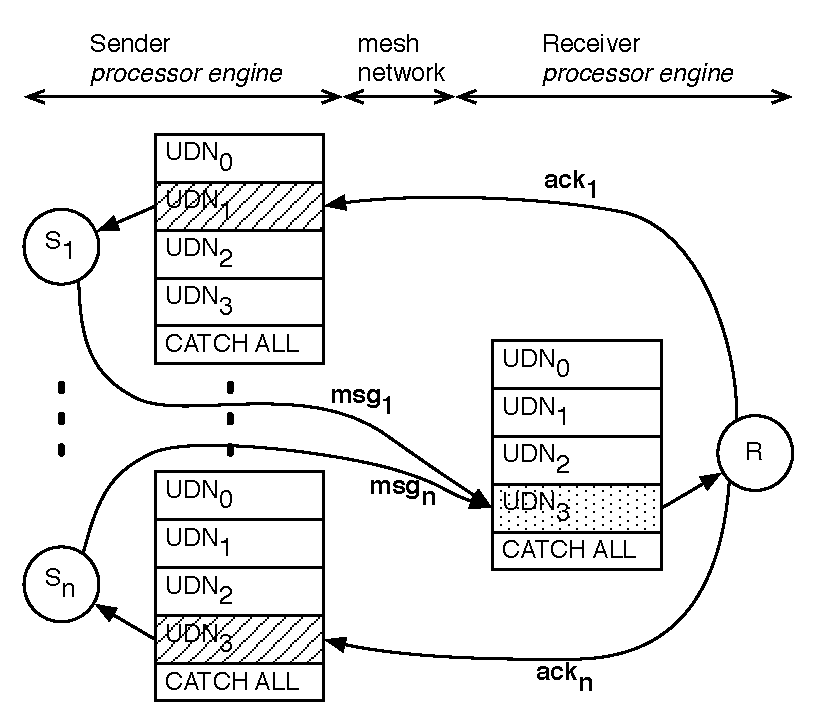
\includegraphics[scale=.5]{udn_asym.pdf}
  \caption[Comunicazione asimmetrica su UDN]{Rappresentazione di un possibile scenario di comunicazione asimmetrica in ingresso tra l'insieme di processi mittenti $\{ S_1, \dots, S_n \}$ e il processo destinatario R, sfruttando la UDN}
  \label{fig:udn_asym}
\end{figure}
L'implementazione della comunicazione asimmetrica in ingresso deriva da quella simmetrica: un generico processo mittente del canale dispone di una coda UDN sulla quale legge gli eventi di Ack, il processo ricevente del canale usa una singola coda UDN sulla quale legge il messaggio di uno qualsiasi tra i processi mittenti. Un messaggio inviato da un mittente \`e costituito da una coppia di valori: una parola di intestazione contenente l'identificatore del mittente all'interno del canale, e una seconda parola contente il valore del messaggio per il quale \`e stato richiesto l'invio. Il fatto che sia trasmesso anche una intestazione al messaggio \`e trasparente all'utente, in quanto l'esecuzione della ricezione nel processo destinatario rende visibile all'utente solo il valore del messaggio. Come mostrato in figura~\ref{fig:udn_asym} diversi mittenti dello stesso canale possono avere come una coda UDN di ricezione qualsiasi, questo crea un problema simile a quello visto nell'implementazione che sfrutta la memoria condivisa nella sezione~\ref{sct:asymin_sm_rdyack}: durante l'esecuzione della primitiva di invio del canale, da parte di un generico mittente, deve essere noto l'identificatore del mittente all'interno del canale stesso, in modo da sapere quale coda UDN usare per l'evento Ack e che valore dare all'intestazione dei messaggi. Anche per questa implementazione del canale asimmetrico si usa un terzo parametro nella primitiva di invio: l'identificatore nel canale del mittente. Il comportamento del protocollo \`e descritto nel codice~\ref{lst:abstr_udn_asym}; come nel canale simmetrico, il supporto fa uso di un descrittore di canale contenente le informazioni sulle cpu e le code UDN usate dai processi comunicanti, nel caso dei processi mittenti tali informazioni sono organizzate in array accedute con l'identificatore del mittente all'interno del canale.
\begin{lstlisting}[
        float=!h,
        morekeywords={dq_snd, dq_rcv, cpu_snd, cpu_rcv}, 
        caption={Descrizione astratta del protocollo di comunicazione Rdy-Ack su UDN per un canale di comunicazione asimmetrico in ingresso},
        label={lst:abstr_udn_asym}
]
send(ch_descr, msg, rank) ::
  leggi una parola dalla UDN Demux Queue 
    ch_descr->dq_snd[rank]
  invia tramite UDN la sequenza di valori <rank, msg> alla
    UDN Demux Queue ch_descr->dq_rcv del PE
    ch_descr->cpu_rcv

receive(ch_descr) ::
  leggi una parola dalla UDN Demux Queue ch_descr->dq_rcv e
    assega il valore alla variablie sender
  leggi una parola dalla UDN Demux Queue ch_descr->dq_rcv e
    assegna il valore alla variablie targa
  invia tramite UDN una parola arbitraria alla UDN Demux
    Queue ch_descr->dq_snd[sender] del PE 
    ch_descr->cpu_snd[sender]
\end{lstlisting}

L'analisi della correttezza della comunicazione \`e simile a quella descritta nell'implementazione simmetrica: \begin{inparaenum}[\itshape a~\upshape)] \item durante l'implementazione del canale devono essere inviati i messaggi di Ack a tutti i mittenti nelle relative code UDN, \item l'utente si fa carico di non usare in un certo processo, eseguito in modo esclusivo in un PE, la stessa coda UDN per pi\`u canali o compiti diversi\end{inparaenum}. Si osserva inoltre che l'unit\`a di routing di UDN \`e il pacchetto \cite{ug101}, quindi l'invio della coppia di parole $<sender_{rank},\;msg>$ da parte di un mittente non viene mai ricevuta intervallata da altre parole nella coda UDN del destinatario se l'invio \`e stato fatto impostando la coppia di parole come payload di un unico pacchetto. Al contrario l'invio di due pacchetti UDN per l'invio della coppia risulta non corretto per l'implementazione descritta.

Si analizza infine la possibilit\`a di situazioni di deadlock causate dall'uso della UDN, che come descritto nella sezione~\ref{sct:intro_arch_udn} \`e soggetta a tale problema. Anche in questo caso l'uso di un paradigma di comunicazione client-server, con un protocollo caratterizzato da grado di asincronia unitario nega il verificarsi di qualsiasi situazione di deadlock (con le ipotesi di correttezza precedenti). Il supporto della comunicazione \`e infatti caratterizzato da un comportamento client-server con interazione domanda-e-risposta, in cui il servente \`e il destinatario e i mittenti sono i clienti. Le richieste dei clienti sono i messaggi inviati dai clienti e le risposte sono i messaggi di ack inviati dal destinatario. In una computazione di questo tipo il deadlock avviene soltanto se i messaggi di risposta del servente riempono la coda di un cliente, ci\`o accade solo quando un cliente invia pi\`u richieste della capacit\`a della coda UDN di memorizzare le risposte \cite{ug205}.

\FloatBarrier
\subsubsection{Comunicazioni con grado di asincronia maggiore di 1}
\label{sct:ad_gt_1_udn}
Le due implementazioni dei canali simmetrici e asimmetrici che sfruttano UDN si prestano ad essere estese ad un grado di asincronia maggiore di uno, \`e infatti sufficiente inviare un numero $m > 1$ di messaggi di Ack al/i mettente/i in fase di inizializzazione del canale. In questo modo eseguendo lo stesso protocollo precedentemente definito si ha un comportamento asincrono di grado $m$. 

Occorre porre attenzione al fatto che un grado di asincronia elevato pu\`o causare il deadlock dell'applicazione. In particolare un mittente non deve inviare pi\`u messaggi della dimensione della coda di demultiplexing UDN. Dato che in entrambe le forme di canale le risposte del destinatario hanno dimensione una parola allora il massimo grado di asincronia \`e la dimensione delle code UDN, per entrambi i canali.

\FloatBarrier
\subsubsection{Implementazione generica}
\label{sct:generic_udn}
Non \`e fornita una implementazione dei canali che sfrutti la UDN e che non limiti per ogni processo il numero di canali utilizzabili. Si descrive qui una possibile implementazione. La limitazione fisica di un numero finito di canali UDN \`e superata utilizzando, con il paradigma precedente, per pi\`u canali ``software'', almeno una coda UDN nel mittente e nel destinatario. I diversi canali ``software'' sono riconosciuti mediante una intestazione ai dati scambiati contenente l'identificatore del canale. \`E necessario ricorrere alla memoria condivisa nel caso in cui il processo destinatario invochi la ricezione su un certo canale e i dati ricevuti dalla coda UDN siano appartenenti ad un altro canale ``software'', perci\`o si memorizzano tali dati per un utilizzo successivo e si continua a testare la coda UDN in attesa dei dati del canale usato. 

Si suppone che una implementazione di questo tipo sia sempre usata insieme all'implementazione ``specializzata su UDN'', pu\`o essere quindi conveniente lasciare le quattro code UDN di demultiplexing a quest'ultima implementazione, e usare la coda \emph{catch all} per l'implementazione ``generica su UDN''. Tale coda viene usata quando si inviano pacchetti UDN con tag di demultiplexing diverso dai quattro valori delle code firmware, la ricezione viene effettuata mediante la lettura di registri SPR. 

L'uso di una implementazione ``UDN generica'' pu\`o essere una utile alternativa alla implementazione che sfrutta esclusivamente la memoria condivisa (descritta in \ref{sct:specifica_sm}) per applicazioni che necessitano di pi\`u di quattro canali per processo e basse latenze di comunicazione. Si osserva tuttavia che pi\`u sono usati molti canali di comunicazione in un singolo processo, pi\`u aumenta la probabilit\`a di ricevere il messaggio di un canale diverso e quindi la necessit\`a di eseguire una copia in memoria (overhead).


